% !TEX root=../presentation_1.tex
\section{Method}

\begin{frame}
\frametitle{A Simple Deterministic Algorithm [Elk17]}
\begin{itemize}
    \item Idea: use better BFS broadcasting structure.
    \item Like \textbf{GHS}, still merging components, but now use an auxillary BFS tree to coordinate - $O(D)$.
    \item Suppose we have an $(n/k,O(k))$-MST forest $\mathcal{F}$ using GHS. 
    \item At most $n/k$ fragments, diameter $O(k)$.
    \item $O(k \log^*n)$ rounds with $O(m + k \log n)$ messages.
\end{itemize}
\end{frame}

\begin{frame}
\frametitle{A Simple Deterministic Algorithm [Elk17]}
\begin{itemize}
    \item Build an auxillary BFS tree $\tau$.
    \item $O(D)$ time and $O(m)$ messages.
    \item Each node compute the BFS interval.
    \begin{itemize}
        \item One convergecast to count the number of leaves under each node.
        \item One broadcast to assign interval.
        \item $O(D)$ time and $O(n)$ messages.
    \end{itemize}
    \item Interval is computed so that we know how to route messages from the root to any base fragment F
\end{itemize}
\begin{figure}
\centering
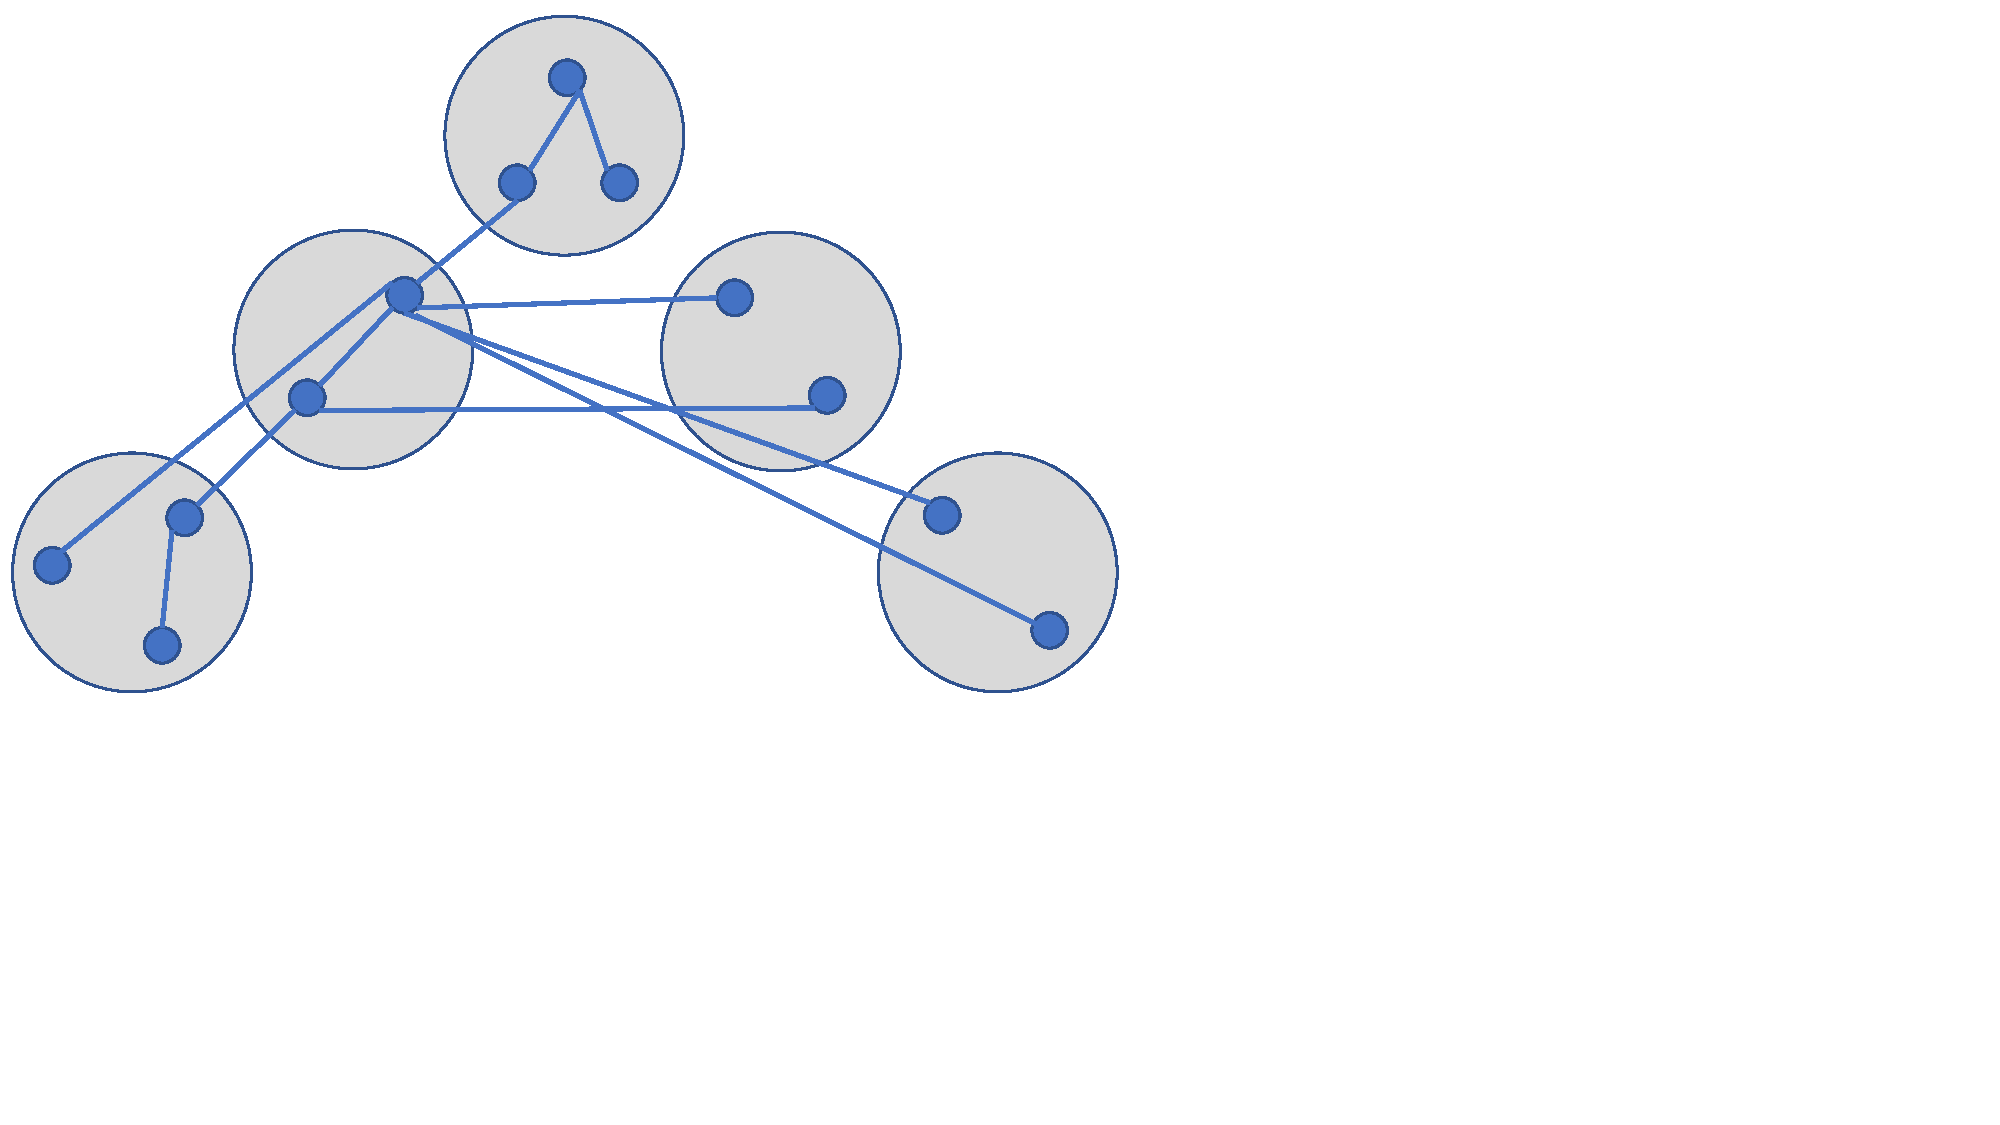
\includegraphics[width=0.4\textwidth,trim={0cm 5cm 12cm 0},clip]{figures/bfstree.pdf}
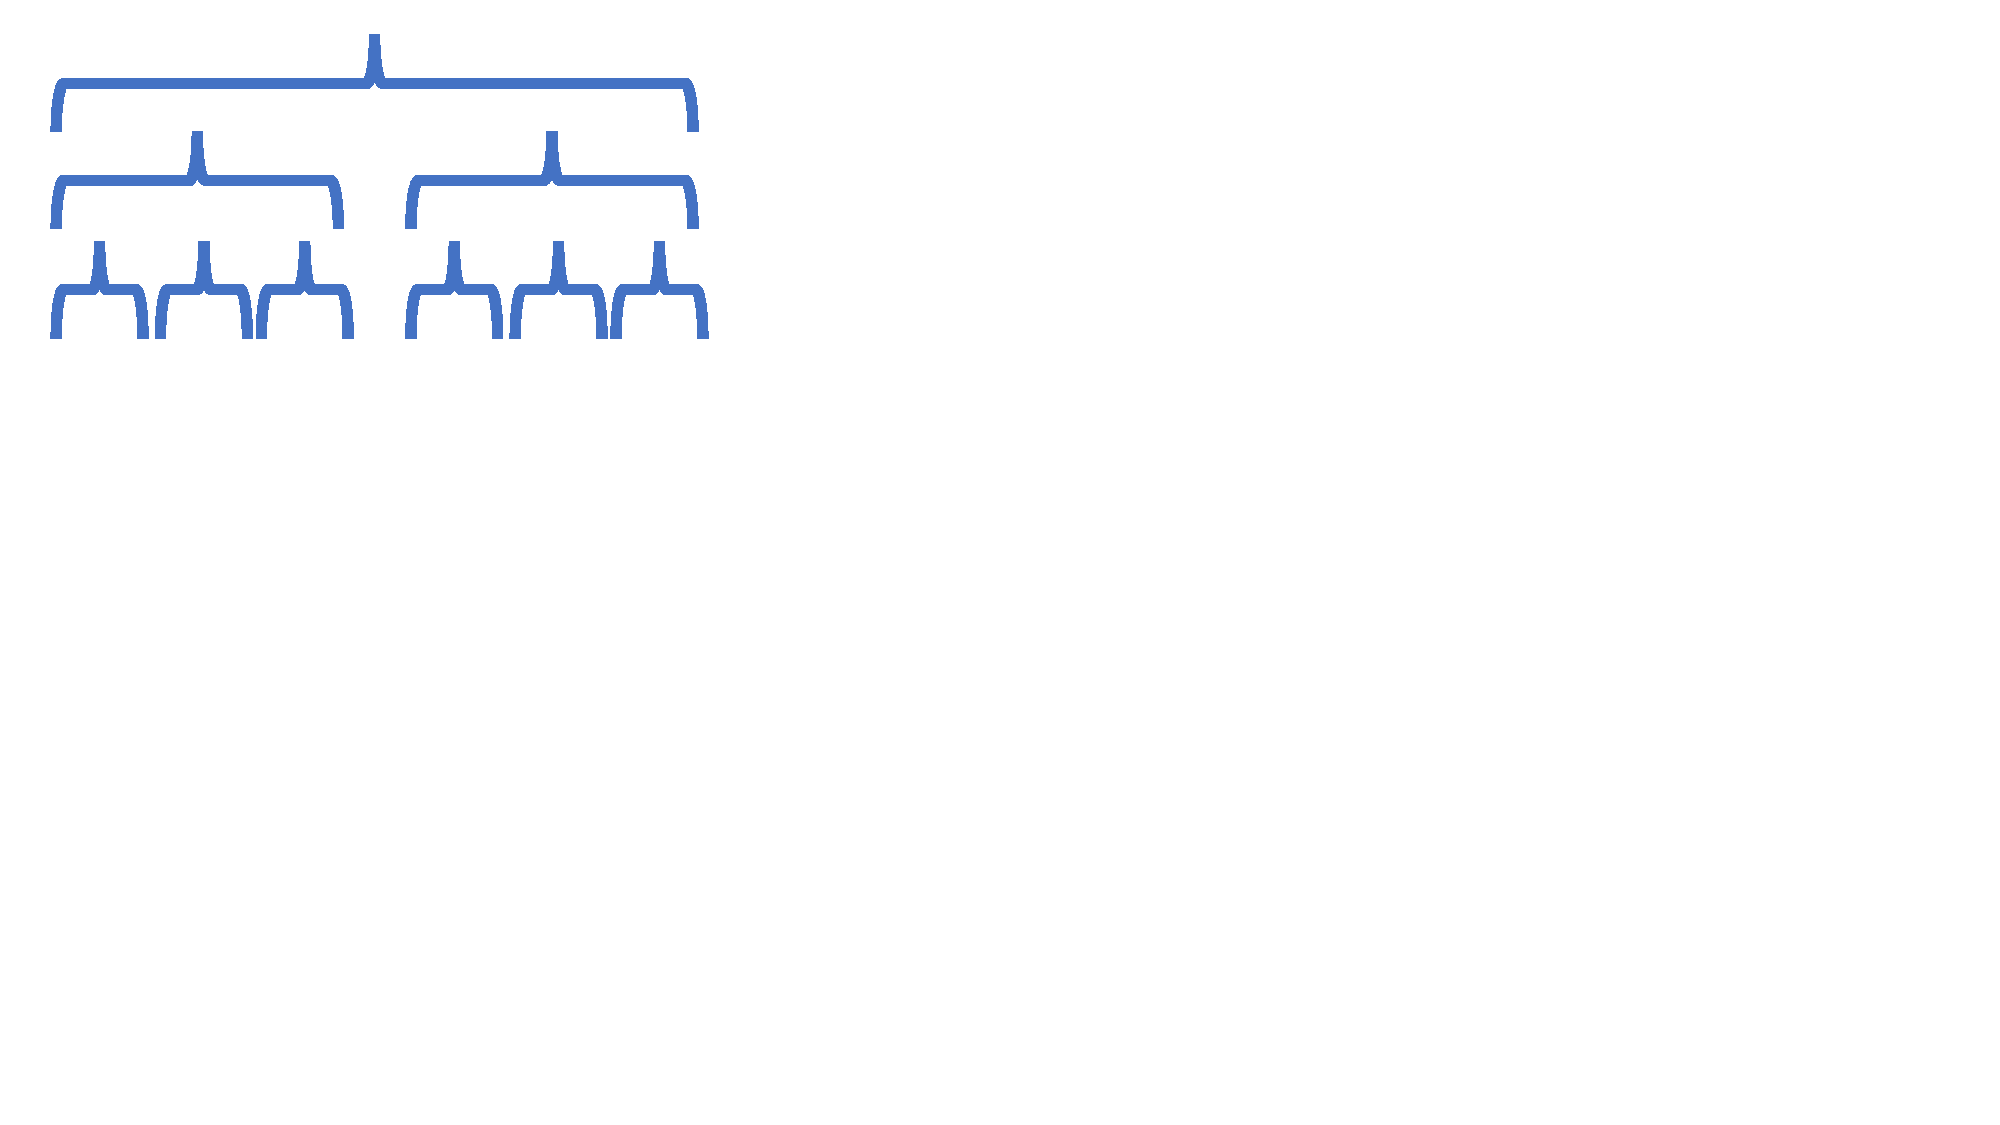
\includegraphics[width=0.4\textwidth,trim={0cm 10cm 20cm 0},clip]{figures/interval.pdf}
\end{figure}
\end{frame}

\begin{frame}
\frametitle{A Simple Deterministic Algorithm [Elk17]}
\begin{itemize}
    \item Finally conduct a pipelined convergecast and the root learns the intervals of all the base fragments. Sends messages of the maximum interval of each fragment.
    \item Takes $O(D+\frac{n}{k})$ and $O(D \cdot \frac{n}{k})$ messages. (Need to aggregate messages of one fragment at a time.)
\end{itemize}
\end{frame}

\begin{frame}
\frametitle{A Simple Deterministic Algorithm [Elk17]}
\begin{itemize}
    \item To send the fragment ID: $O(1)$ rounds and $O(m)$ messages.
    \item To convergecast the $\frac{n}{k}$ fragment IDs: $O(D+\frac{n}{k})$ rounds and $O(D \cdot\frac{n}{k})$ messages.
    \item Assume each vertex knows its fragment ID, and also the fragments IDs of its neighbors
    \item We can compute MWOE locally, and send to the root of the fragment
    \item Now suppose $D \le \sqrt{n}$, and we select $k=\sqrt{n}$.
    \item $O(k)=O(\sqrt{n})$ rounds and $O(n)$ messages.
\end{itemize}
\end{frame}

\begin{frame}
\frametitle{A Simple Deterministic Algorithm [Elk17]}
\begin{itemize}
    \item Perform a \textbf{pipelined convergecast} to the root, send MWOE of each component.
    \item $O(D+\frac{n}{k})$ rounds and $O(D \cdot \frac{n}{k})$ messages.
    \item Then the root tells each fragment which one to merge with.
    \item Sends message $<F,F'>$ through pipelined broadcast, to tell $F$ to merge with $F'$.
    \item The node that receives merge message, changes the fragment ID.
    \item $O(D+\frac{n}{k})$ rounds and $O(D \cdot \frac{n}{k})$ messages.
\end{itemize}
\end{frame}

\begin{frame}
\frametitle{A Simple Deterministic Algorithm [Elk17]}
\begin{itemize}
    \item Finally, every vertex notifies its neighbors about the change in fragment ID. 
    \item $O(1)$ rounds and $O(m)$ messages.
    \item Round: $O(D+\frac{n}{k}) + O(k\log^* n) + O((D + k + \frac{n}{k})\log n) = O(\sqrt{n}\log n)$.
    \item Message: $O(E \log n + n\log n \cdot \log^* n)$
\end{itemize}
\end{frame}

\begin{frame}
\frametitle{A Simple Deterministic Algorithm [Elk17]}
\begin{itemize}
    \item If $D > \sqrt{n}$, then let $k=D$.
    \item $O(D+\frac{n}{k}) + O(k\log^* n) + O((D + k + \frac{n}{k})\log n) = O(D\log n)$ rounds
    \item The number of messages is the same as before.
    \item Round: $O((D + \sqrt{n})\log n)$
    \item Message: $O(E \log n + n\log n \cdot \log^* n)$
\end{itemize}
\end{frame}


\begin{frame}
\frametitle{Conclusion}
\begin{itemize}
    \item Near optimal time and message complexities.
    \item A fully deterministic algorithm.
\end{itemize}

% !TEX root=../presentation_1.tex
\begin{table}
\renewcommand{\arraystretch}{1.3}
\caption{Summary of the complexity of distributed MST algorithms}
\begin{tabular}{|c|c|c|}
\hline
Method         & Time Complexity            & Message Complexity\\
\hline
\hline
Pipeline-MST   & $O(D + n)$                 & $O(m + n^2)$\\
\hline
GHS            & $O(n \log n)$              & $O(m + n \log n)$\\
\hline
Controlled-GHS & $O(D + \sqrt{n} \log^* n)$ & $O(m + n^{\frac{3}{2}})$\\
\hline
\textbf{This Work}& $O((D + \sqrt{n}) \log n)$  & $O(m \log n + n \log n \log^* n)$ \\
\hline
\hline
Randomized [PRS16]& $\tilde{O}(D + \sqrt{n})$  & $\tilde{O}(m)$ \\
\hline
Lower Bound [PRS16] & $\tilde{\Omega}(D + \sqrt{n})$  & $\Omega(m)$ \\
\hline
\end{tabular}
\end{table}

\end{frame}
